\section{Class Diagram for movement}

On \ref{ClassDiagramMovement} the simplified class diagram is shown it shows how moving a player works. The central part of the diagram is the GameView which is holding the game state lists. These lists control where players, monsters and items are on the map. Each class displayed holds a greater number of functions and attributes but they have been cleared for simplicity, showing only the relevant things for movement and general understanding.


\begin{figure}
	\centering
	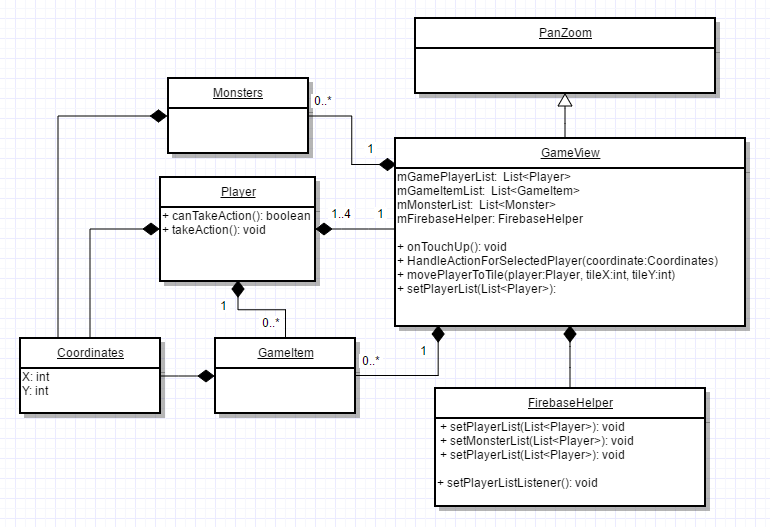
\includegraphics[width=0.8\textwidth]{images/ClassDiagramMovement.PNG}
	\caption{Class Diagram for movement of player \label{ClassDiagramMovement}}
\end{figure}